\documentclass{article}
\usepackage{microtype}
\usepackage{graphicx}
\usepackage{subfigure}
\usepackage{booktabs} 
\usepackage{hyperref}
\usepackage{spreadtab}
\usepackage{xspace}
\usepackage{amsfonts, amsmath}
\usepackage{pgfplots}
\usepackage{multirow}

\newcommand{\theHalgorithm}{\arabic{algorithm}}
\usepackage{sysml2019}

\sysmltitlerunning{Practical Continuous Integration for Machine Learning}

\begin{document}

\twocolumn[
\sysmltitle{ease.ml/ci: Towards Rigorous but Practical Continuous Integration for Machine Learning Workloads}

\sysmlsetsymbol{equal}{*}

\begin{sysmlauthorlist}
\sysmlauthor{Aeiau Zzzz}{equal,to}
\sysmlauthor{Bauiu C.~Yyyy}{equal,to,goo}
\sysmlauthor{Cieua Vvvvv}{goo}
\sysmlauthor{Iaesut Saoeu}{ed}
\sysmlauthor{Fiuea Rrrr}{to}
\sysmlauthor{Tateu H.~Yasehe}{ed,to,goo}
\sysmlauthor{Aaoeu Iasoh}{goo}
\sysmlauthor{Buiui Eueu}{ed}
\sysmlauthor{Aeuia Zzzz}{ed}
\sysmlauthor{Bieea C.~Yyyy}{to,goo}
\sysmlauthor{Teoau Xxxx}{ed}
\sysmlauthor{Eee Pppp}{ed}
\end{sysmlauthorlist}
\sysmlaffiliation{to}{Department of Computation, University of Torontoland, Torontoland, Canada}
\sysmlaffiliation{goo}{Googol ShallowMind, New London, Michigan, USA}
\sysmlaffiliation{ed}{School of Computation, University of Edenborrow, Edenborrow, United Kingdom}
\sysmlcorrespondingauthor{Cieua Vvvvv}{c.vvvvv@googol.com}
\sysmlcorrespondingauthor{Eee Pppp}{ep@eden.co.uk}

\vskip 0.3in

\begin{abstract}
Blah blah
\end{abstract}
]

% this must go after the closing bracket ] following \twocolumn[ ...

% This command actually creates the footnote in the first column
% listing the affiliations and the copyright notice.
% The command takes one argument, which is text to display at the start of the footnote.
% The \sysmlEqualContribution command is standard text for equal contribution.
% Remove it (just {}) if you do not need this facility.

%\printAffiliationsAndNotice{}  % leave blank if no need to mention equal contribution
\printAffiliationsAndNotice{\sysmlEqualContribution} % otherwise use the standard text.




%\documentclass{vldb}
%\usepackage[utf8]{inputenc}
%
%\usepackage{spreadtab}
%\usepackage{xspace}
%\usepackage{amsfonts, amsmath}
%\usepackage{pgfplots}
%\usepackage{multirow}
%
\newcommand{\sys}{\texttt{ease.ml/ci}\xspace}

%\vldbTitle{ease.ml/ci: Rigorous, Practical, and Declarative Continuous Integration for Machine Learning Workloads}
%\vldbAuthors{}
%\vldbDOI{https://doi.org/TBD}
%\vldbVolume{12}
%\vldbNumber{xxx}
%\vldbYear{2019}

%\begin{document}

%\title{ease.ml/ci: Rigorous, Practical, and Declarative Continuous Integration for Machine Learning Workloads}
%\maketitle

\begin{figure}[t!]
\centering
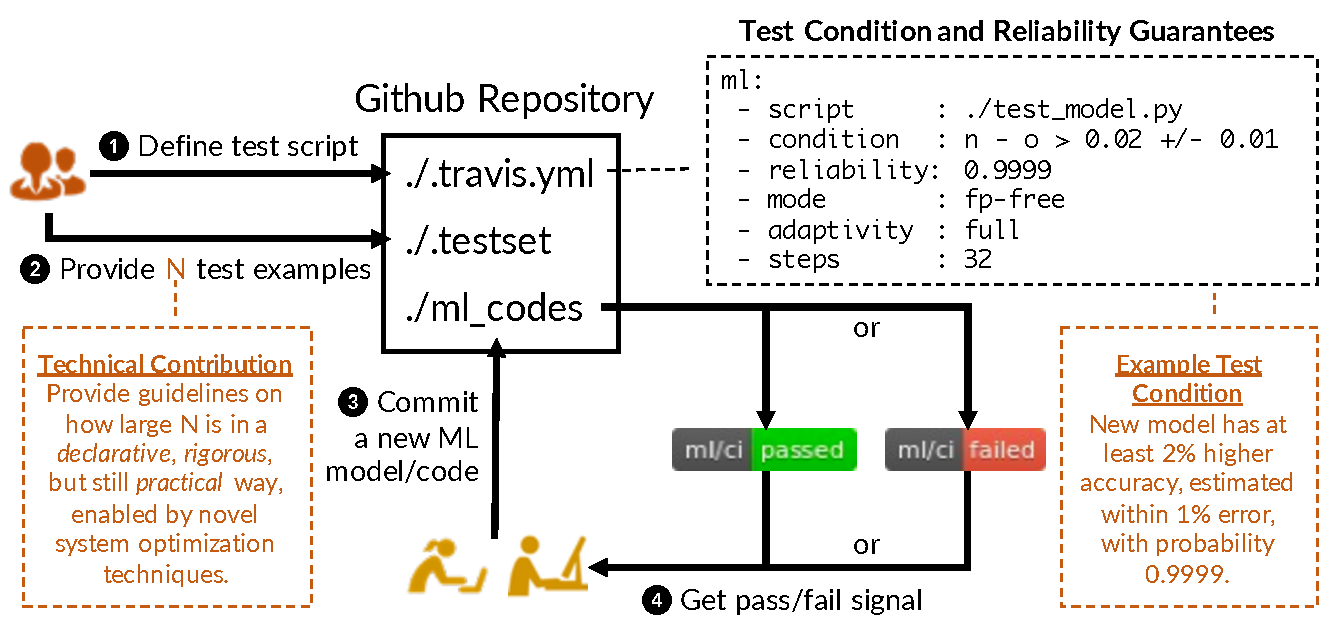
\includegraphics[width=0.5\textwidth]{figures/CI.pdf}
\vspace{-2em}
\caption{\sys is a {\em continuous integration system}
for machine learning. It supports a four-step
workflow: (1) user describes in a {\em test configuration script} containing
the test conditions with respect to the quality
of a ML model; (2) user provides $N$ test
examples where $N$ is automatically calculated
by the system given the configuration script; (3) whenever developer commits/checks in 
an updated ML model/program, the
system triggers a build; and (4) the 
system tests whether the test condition is
satisfied and returns a pass/fail signal
to the developer. When the current test set
loses its ``statistical power'' due to repetitive evaluation, the system also decides
on when to request from 
the user a new testset. The technical contribution
of this work is a new set of techniques
that enables a practical $N$
(e.g., 10K-20K test examples) with
strong, rigorous theoretical guarantees
(e.g., estimation error within 1\% accuracy, with 0.9999 probability, in an adaptive 
scenario).}
\label{fig:e2e}
\end{figure}

\section{Introduction}

\vspace{1em}
\noindent
{\bf (What is Practical?)} The practicality 
is user dependent. From our experience working
with different users, we observe that 
providing $28,800$ labels for every $32$ model
evaluations seems to be a pretty easy sell 
for most of the users: $28,800$ is what two
engineers can label in a day (8 hours) with a
rate of 2 seconds per label, and 32 model evaluations
means one commits per day. Under this assumption, the user only
only need to spend one day per month to provide
test labels. This is what most of our users 
find reasonable.

\section{System Design}

\subsection{Interaction Model}


\subsection{A \sys Script}

The goal of \sys is to provide a declarative way for users
to specify the requirements of a new machine learning model
to pass the continuous integration test, and compiles
it to a {\em practical} workflow to enable such tests with
rigorous theoretical guarantees. We first describe,
at the logical level, the design of an \sys script, and
then describe the physical implementation of this script
as an extension to the \texttt{.travis.yml} file
used in Travis CI.

\paragraph*{Logical Data Model} The core part of an \sys
script is a user-specified condition for the continuous
integration test. In the current version, such a condition
is specified over three variables $\mathcal{V} = \{n, o, d\}$:
(1) $n$, the accuracy of the new model, (2) $o$ the
accuracy of the old model, and (3) $d$, the percentage
the predictions of the new model that is different from 
the old model. $\{n, o, d\} \in [0, 1]$.

\paragraph*{Syntax of a Condition}
To specify the condition, which will be tested by
\sys whenever a new model gets committed, the user
uses the following syntax:
\begin{verbatim}
      c   :- floating point constant
      v   :- n | o | d
      op1 :- + | -
      op2 :- *
      EXP :- v | v op1 EXP | EXP op2 c

      cmp :- > | < 
      C   :- EXP cmp c +/- c

      F   :- C | C /\ F
\end{verbatim}
\texttt{F} is the final condition, which is a 
conjunction of a set of clauses \texttt{C}.
Each clause is a comparison between a 
algebraic expression over $\{n, o, d\}$
and a constant, with an error tolerance 
following the symbol \texttt{+/-}.

For example, two expressions that we focus
on optimizing in this paper can be specified
as follows:
\begin{verbatim}
      n - o > 0.02 +/- 0.01 /\ d < 0.1 +/- 0.01
\end{verbatim}
in which the first clause
\begin{verbatim}
                n - o > 0.02 +/- 0.01
\end{verbatim}
requires that the new model has an accuracy that is
two points higher than the old model, with the error
tolerance of the estimation to be 1 point of accuracy,
while the clause
\begin{verbatim}
                   d < 0.1 +/- 0.01
\end{verbatim}
requires that the new model only changes 10\%
of the predictions made by the old model, with the
tolerance of the estimation to be 1 point.

\paragraph*{Semantics of Continuous Integration Tests}
Different from traditional continuous integration,
all three variables used in \sys, i.e., $\{n, o, d\}$,
are {\em random variables}. As a result, the 
checking of an \sys condition is inherently {\em probabilistic}. There are two additional parameters
that the user needs to provide, which would decide 
the semantics of the test condition: (1) $\delta$,
the probability with which the test process is allowed 
to be incorrect, which is usually chosen to be smaller
than 0.001 or 0.0001 (i.e., 0.999 or 0.9999 success rate); and (2) \texttt{mode} chosen from
\texttt{\{fp-free, fn-free\}}, which specifies 
whether the test is {\em false-positive free} or
{\em false-negative free}. Given these two parameters,
to semantics of \sys is to ensure that 
with probability $1 - \delta$, the output of 
\sys is free of false positives or false negatives.

The notion of false positives or false negatives
is related to the fundamental trade off between
the ``type I'' error and the ``type II'' error
in statistical hypothesis testing.
Consider the following simple condition
\begin{verbatim}
                   x < 0.1 +/- 0.01
\end{verbatim}
and the real {\em unknown} value of $x$ to be
$x^*$. Given an estimator $\hat{x}$, which,
with probability $1-\delta$, satisfies
$\hat{x} \in [x^* - 0.01, x^* + 0.01]$, how can we 
give an answer to this condition?
\begin{enumerate}
\item When $\hat{x} > 0.11$, clearly the condition
returns \texttt{False} as the real value $x^*$
is impossible to be smaller than 0.1, with 
probability $1-\delta$.
\item When $\hat{x} < 0.09$, clearly the condition
returns \texttt{True} as the real value $x^*$
is impossible to be larger than 0.1, with 
probability $1-\delta$.
\item When $0.09 < \hat{x} < 0.11$, we cannot 
gives a definite answer to the condition --- even if
$\hat{x} > 0.1$, there is no way to we can tell
whether the real value $x^*$ is larger or smaller
than 0.1. In this case, the condition evaluates to
\texttt{Unknown}.
\end{enumerate}

The parameter \texttt{mode} provides the way for
the system to deal with the case that the condition
evaluates to \texttt{Unknown} --- In
\texttt{fp-free} mode, \sys treats \texttt{Unknown}
as \texttt{False} (thus reject the commit) to ensure
that whenever the condition evaluates to \texttt{True}
using an estimator, the real underlying variable 
always evaluate to \texttt{True} for the same condition. 
Similarly, in \texttt{fn-free} mode, 
\sys treats \texttt{Unknown}
as \texttt{True} (thus accept the commit).
The false positive rate (resp. false negative rate)
in the \texttt{fn-free} (resp. \texttt{fp-free})
mode is specified by the error tolerance parameter.

\paragraph*{Adaptive vs. Non-adaptive Integration}
Another prominent difference between \sys and 
traditional continuous integration system is that 
the statistical power of a test dataset would decrease
the moment that the result of whether a new model
passes the continuous integration test being released
to the developer: In this case, the developer could
adaptively engineers the next model to increase the
probability that it passes the test. This
is related to the recent theoretical 
analysis on adaptive analytics~\cite{XXX,XXX}.
As we will see, supporting adaptive development
is more expensive and it requires a larger test set.

As a system, \sys needs to provide the same level
of guarantee given the worst case user behavior.
In the current system, \sys allows the user to specify
whether the test is adaptive or not
with a flag \texttt{adaptivity} (\texttt{full},
\texttt{none}, \texttt{firstSuccess}). 
When the test is \texttt{full},
the system releases the information of whether 
the new model passes the test immediately to the developer;
when the test is \texttt{none}, the system accepts
all commits, however, sends the information of
whether the model really passes the test to
a user-specified, third-party, email address.
The adaptivity level \texttt{firstSuccess}
allows full adaptivity before the first time
that the developer passes the test, and stops
afterwards and requires a new test set (See Section~\ref{sec:adaptive}).

\paragraph*{Physical Implementation}
An \sys script is implemented as an 
extension to the \texttt{.travis.yml} file
used in Travis CI by adding a \texttt{ml} section.
For example,
\begin{verbatim}
      ml:
        - script     : ./test_model.py 
        - condition  : n - o > 0.02 +/- 0.01 
        - reliability: 0.9999
        - mode       : fp-free
        - adaptivity : full
        - steps      : 32
\end{verbatim}
This script specifies a continuous test process
that, with probability larger than 0.9999,
accepts the new commit only if the new model 
has two points higher accuracy than the old
model. This estimation is conducted with an 
estimation error within one accuracy point
in a false positive-free manner. The system 
will release the test result immediately,
and the user expects that the given test set
will be used at most by 32 times before
a new test set be provided to the system.

Similarly, if the user wants to specify a 
non-adaptive integration process, she can provide
a script as follows
\begin{verbatim}
      ml:
        - script     : ./test_model.py 
        - condition  : d < 0.1 +/- 0.01
        - reliability: 0.9999
        - mode       : fp-free
        - adaptivity : none -> contact@examples.com
        - steps      : 32
\end{verbatim}
which accepts each commit but sends
the test result to the email address 
contact@examples.com after every commit.

\paragraph*{Discussion and Future Extensions}
The current syntax of \sys is able to model 
many realistic use cases that our users find
useful in their own development process, 
which includes to reason about the difference
of accuracy between the new model and the old model,
and to reason about the amount of changes 
between the new and old model. In principle,
\sys could supports a richer syntax.
We list some limitations of the current
syntax that we believe are interesting directions
for future research.
\begin{enumerate}
\item Beyond Accuracy: There are other important
quality metrics for machine learning that the current
system does not support, i.e., F1-score, AUC score, etc.
\item Ratio Statistics: The current syntax of \sys
intentionally leaves out division \texttt{/} and it
would be useful for a future version to enable the 
relative comparison of quality.
\item Order Statistics: In our experience, some users
think that order statistics are also useful, e.g.,
to make sure the new model is within the top-5 models
in the development history.
\end{enumerate}
The current version of \sys does not provide the support
for all these features. However, we believe that many
of them could be supported by developing similar statistical
techniques as we did for the current version of \sys.
As the first continuous integration system for ML,
supporting even the simple syntax requires careful
design of the system architecture and the development
of novel techniques. As a result, we focus on 
a simplified version that is enough to support the 
top requirements from our users, and leave these
extensions to future work.

\subsection{System Utilities}

Different from traditional continuous integration,
in which the system can safely assume that the user
has the knowledge and competency to build the test
suite all by herself, this assumption is too strong
for \sys. One of the most prominent conceptual 
contribution of \sys is a collection of techniques
that provide practical, but rigorous, guidelines 
for the user to manage the test set: {\em How large
does the test set need to be?} {\em When does the system need
a new freshly generated test set?} {\em When can
the system release the test set and ``downgrade''
it into a development set?} While most of these
questions are answered by experts with heuristics
and intuition, the goal of \sys is to provide 
systematic, principled guidelines.

As a result, \sys provides two utilities 
that are not provided in systems such as Travis CI.

{\bf (Sample Size Estimator)} The sample size estimator is a program that takes
as input a \sys script, and outputs the number of
examples that the user needs to provide as the test
set. 

{\bf (New Testset Alert)}
The new testset alert subsystem is a program
that takes as input a \sys script the 
the the commit history of machine learning models,
and produces an alert (e.g., by 
sending an email) to the user when the current
test set has been used too many times and thus cannot
be used to test the next committed model.
Upon receiving the alert, the user needs to provide 
a new test set to the system and can also release the old
testset to the development team.


An impractical implementation of these two ultilities
are easy --- the system alerts the users to request
a new test set after every commit and estimate the
sizes of the test set simply using the Hoeffding bound.
However, to make \sys a useful tool for real-world 
users, these utilities need to be implemented in 
a more practical way. The technical contribution of
\sys is a set of techniques, which could reduce 
the number of samples the system requests from the user
by up to two orders of magnitude.

\section{Baseline Implementation}

We describe the techniques to implement 
\sys for user-specified conditions in the
most general case. The techniques that we
use involve standard Hoeffding inequality
and a technique similar to Ladder~\cite{XXX}
in the adaptive case. This implement is
general enough to support all user-specified conditions
currently allowed in \sys, however, could 
be made more practical when the test conditions
satisfy certain conditions. We leave the 
system optimizations for specific conditions
to Section~\ref{sec:opt}.

\subsection{Sample Size Estimator for a Single Model}

\paragraph*{Estimator for a Single Variable}
One building block of \sys is the estimator of
the number of samples one needs to estimate 
one variable ($n$, $o$, and $d$) to $\epsilon$
accuracy with $1-\delta$ probability. We construct
this estimator with the standard Hoeffding bound.

A sample size estimator $n: \mathcal{V} \times [0-1]^3 \mapsto \mathbb{N}$ is a function that takes as input
a variable, its dynamic range, error tolerance, and
success rate, and outputs the number of samples 
one need in the test set. With standard Hoeffding:
\[
n(v, r_v, \epsilon, \delta) = \frac{-r_v^2 \ln \delta}{2\epsilon^2}
\]
where $r_v$ is the dynamic range of the variable 
$v$, $\epsilon$ the error tolerance, and 
$1-\delta$ the success probability.

\paragraph*{Estimator for a Single Clause}

Given a clause $C$ with a left-hand side expression
$\Phi$, a comparison operator $cmp$, and a right-hand
side constant, the sample size estimator returns the
number of samples one need to provide an 
$(\epsilon, \delta)$-estimation of the left-hand side 
expression. This can be done with a 
trivial recursion:
\begin{enumerate}
\item $n(\texttt{c * v}, \epsilon, \delta) = n(v, r_v, \epsilon / c, \delta)$ where $c$ is a constant. As a result, we have
\[
n(\texttt{c * v}, \epsilon, \delta) = \frac{- c^2 r_v^2 \ln \delta}{2\epsilon^2}.
\]
\item $n(\texttt{EXP1 + EXP2}, \epsilon, \delta) =
   \max \{n(\texttt{EXP1}, \epsilon_1, \frac{\delta}{2}),
          n(\texttt{EXP2}, \epsilon_2, \frac{\delta}{2})\}$
where $\epsilon_1 + \epsilon_2 < \epsilon$. The same
equality holds similarly for
$n(\texttt{EXP1 - EXP2}, \epsilon, \delta)$.
\end{enumerate}

\paragraph*{Estimator for a Single Formula}

Given a formula $F$ which is a conjunction over
$k$ clauses ${C_1, ..., C_k}$, the sample size
estimator needs to guarantee that it can 
satisfies each of the clause $C_i$. One way
to build such an estimator is as follows:
\[
n(\texttt{F}, \epsilon, \delta) = \max_i n(C_i, \epsilon, \frac{\delta}{k}).
\]

\paragraph*{Example} Given a formula $F$, we now have a simple algorithm for sample size estimation. 
For example, for the following formula 
\begin{verbatim}
F :- n - 1.1 * o > 0.01 +/- 0.01 /\ d < 0.1 +/- 0.01    
\end{verbatim}
the system will translate it into an
optimization problem
\[
n(\texttt{F}, \epsilon, \delta) = 
\min_{\substack{
\epsilon_1 + \epsilon_2 = \epsilon\\ \epsilon_1, \epsilon_2 \in [0, 1]}}
\max\{
\frac{- \ln \frac{\delta}{4}}{2\epsilon_1^2},
\frac{- 1.1^2 \ln \frac{\delta}{4}}{2\epsilon_2^2},
\frac{- \ln \frac{\delta}{2}}{2\epsilon^2}
\}
\]
and solve it using projected subgradient descent.

\subsection{Non-Adaptive Scenarios}

In the non-adaptive scenario, the system evaluates 
$H$ models, without releasing the result to 
the developer. In \sys, this is implemented by
accepting all commits form the developer while
sending the result to an email address.

\paragraph*{Sample Size Estimation} The sample
size estimation is easy in this case as all
$H$ models are independent. In this case,
to ensure that, with probability $1-\delta$,
\sys returns the right answer for each of the
$H$ models, the number of samples one need
for formula $F$ is simply
\[
n(\texttt{F}, \epsilon, \frac{\delta}{H}).
\]
This follows the standard union bound. 
Therefore, given the number of models that
user hopes to evaluate (specified 
in the \texttt{steps} field in a \sys script),
the system can return the number of samples
necessary in the testset.

\paragraph*{New Testset Alert} The alert 
for users to provide a new testset is
easy to implement in the non-adaptive scenario.
The system maintains a counter of how many 
times the testset has been used. When 
this counter reaches the pre-defined 
budgets (i.e., \texttt{steps}), the system
requests a new testset from the user.
In the meantime, the old testset can be 
released to the developer for future development
process.

\subsection{Fully-Adaptive Scenarios}

In the fully-adaptive scenario, the system releases
the test result (a single bit representing pass/fail)
to the developer. Because this bit leaks the information
of the testset to the developer, one cannot use
union bound anymore as in the non-adaptive scenario.

\paragraph*{Sample Size Estimation} For the 
most general scenario, \sys uses the following way
to estimate the sample size for a $H$-step 
fully-adaptive scenario. The intuition is simple ---
the develop's decision on the next model only
relies on the history --- for $H$ steps, there are
only $2^H$ different histories. As a result, one
only needs to enforce the union bound on all
these $2^H$ possibilities. Therefore, the number
of samples one needs is
\[
n(\texttt{F}, \epsilon, \frac{\delta}{2^H}).
\]

\paragraph*{Is the Exponential Term too Impractical?} 
Readers might worry about the exponential dependencies
on $H$ for the fully adaptive scenario. However, 
for $H$ that is not too large, e.g., $H=32$, 
the above bound can still lead to practical 
number of samples as the $\frac{\delta}{2^H}$ is
within a logarithm term. As an example, consider the
following simple condition:
\begin{verbatim}
               F :- n > 0.8 +/- 0.05
\end{verbatim}
With $H=32$, we have
\[
n(\texttt{F}, \epsilon, \frac{\delta}{2^H}) = \frac{\ln 2^H - \ln \delta}{2\epsilon^2}.
\]
Take $\delta = 0.0001$ and $\epsilon = 0.05$, 
we have $n(\texttt{F}, \epsilon, \frac{\delta}{2^H}) = 6,279$. Assuming the developer checks in the best model
everyday, this means that every month the user needs
to provide only fewer than seven thousands test samples,
a requirement that is not impractical in most cases.
When $\epsilon = 0.01$, this blows up to $156,955$ which
is less practical -- We will show in Section~\ref{sec:opt}
on how to tighten this bound to make it more practical 
for a sub-family (including this example) of queries.

\paragraph*{New Testset Alert} Similar to the non-adaptive
scenario, the alert of requesting a new test set is 
trivial to implement --- The system requests a new
testset when it reaches the pre-defined budget. At that
point, the system can release the testset to the developer
for future development.

\subsection{Hybrid Scenarios}

One could obtain a better bound on the number of required
samples by constraining the information being released
to the developer. Considering the following scenario:
\begin{enumerate}
\item If a commit fails to pass, returns \texttt{Fail} to the developer;
\item If a commit passes, (1) returns \texttt{Pass} to the developer, and (2) triggers the new testset alert to request
a new testset from the users.
\end{enumerate}
Compared with the fully adaptive scenario, in this
scenario, the user provides new testset immediately
after the developer provides a model that passes the 
test. 

\paragraph*{Sample Size Estimation}
Let $H$ be the maximal
number of steps the system supports.
Because the system will request a new testset
immediately after a model passes the test, the
system is not really adaptive --- as long as the 
developer continues to use the same testset, she
can assumes the last model always fails. Assume
that the user is a deterministic function that
returns a new model given the past history and 
past feedback (a steam of \texttt{Pass}), there are
only $H$ possible states that we need to apply
union bound. This gives us the same bound as 
the non-adaptive scenario:
\[
n(\texttt{F}, \epsilon, \frac{\delta}{H}).
\]

\paragraph*{New Testset Alert} Different from the
previous two scenarios, the system will alert
the user whenever the model she provides passes
the test, or reaches pre-defined budget is, whichever
comes earlier.

\paragraph*{Discussion} At the first glance, it 
might be counter-intuitive that the hybrid scenario,
which leaks information to the developer, has the
same sample size estimator as the non-adaptive case.
Given the maximal number of steps that the testset
supports, $H$, the hybrid scenario cannot always 
finish all $H$ steps as it might require a new testset
in $H' << H$ steps. In other words, different from
the adaptive scenario, the hybrid scenario accommodate
the leaking of information not by adding more samples,
but by decreasing the number of steps that a
testset can support. 

The hybrid scenario is useful when the test is hard to pass.
For example, imagine the following condition: 
\begin{verbatim}
             F :- n - o > 0.1 +/- 0.01
\end{verbatim}
That is, the system only accepts commit that increase the
accuracy by 10 accuracy points. In this case, the developer
might take many developing iterations to get a model
that actually satisfies the condition. As a result, it
is not uncommon to expect that there will be a 
large number of models that cannot pass this test 
before a model passes the test.

\subsection{Evaluating a Condition}

Given a test set that satisfies the number of
samples given by the sample size estimator,
we obtain the estimations of each of the
three variables used in a clause, i.e.,
$\hat{n}$, $\hat{o}$, and $\hat{d}$. Simply
using these estimates to evaluate a condition
might cause both false positives and false negatives.
In \sys, we define a simple algebra over
intervals, which is used to evaluate the left-hand
side of a single clause. As a result, a clause
evaluates to \{\texttt{True}, \texttt{False}, 
\texttt{Unknown}\}. The system then maps
this three-value logic into a two-value logic
given user's choice of either \texttt{fp-free}
or \texttt{fn-free}. 

\subsection{Use Cases and Practicality Analysis}

The baseline implementation of \sys relies on 
standard concentration bounds with simple,
but novel, twists to the specific usecase. 
Despite its simplicity, this simple implementation
can already supports some real-world scenarios 
that many of our users find useful. We summarize 
XXX use cases and analyze the number of samples 
the system required from the user. These 
use cases are summarized from observing the 
requirements from the set of users we have been 
supporting over the last two years, ranging from
scientists at ETH, to real production applications
provided by companies such as Huawei and different 
hospitals. We use $\texttt{[c]}$ and $\texttt{[epsilon]}$
to denote the placeholder of constants.

\vspace{1em}
\noindent 
{\bf (F1: Lower Bound Worst Case Quality)}
\begin{verbatim}
        F1         :- n > [c] +/- [epsilon]
        adaptivity :- full | none
        mode       :- fn-free
\end{verbatim}
This condition is used for quality control to avoid
the cases that the developer accidentally commits a
model that has an unacceptably low quality or
has obvious quality bugs.

We see the use case of this condition in both
fully-adaptive scenario or non-adaptive scenario. We 
do not see obvious use cases for the hybrid scenario
as the expectation is that many models will pass
this condition.

We see most of the use cases of this condition 
need to be false-negative free. This is because 
this condition is popularly used as a filter to
distinguish those very bad cases in which the
existence of false negative is not ideal.

\vspace{1em}
\noindent 
{\bf (F2: Incremental Quality Improvement)}
\begin{verbatim}
        F2         :- n - o > [c] +/- [epsilon]
        adaptivity :- full
        mode       :- fp-free
        ([c] is small)
\end{verbatim}
This condition is used for making sure that the
machine learning application monotonically improves
over time. This is important when the machine
learning application is end user-facing, in which 
it is unacceptable for the quality to drop.
In this scenario, it makes sense for the whole
process to be fully adaptive and false positive-free.

\vspace{1em}
\noindent 
{\bf (F3: Significant Quality Milestones)}
\begin{verbatim}
        F3         :- n - o > [c] +/- [epsilon]
        adaptivity :- firstSuccess
        mode       :- fp-free
        ([c] is large)
\end{verbatim}
This condition is used for making sure that the
repository only contains significant quality
milestones (e.g., log models every 10 points
of accuracy jump). Although the condition is
syntactically the same as \texttt{F2}, in this
scenario, it makes sense for the whole
process to be hybrid adaptive and false positive-free.

\vspace{1em}
\noindent 
{\bf (F4: No Significant Changes)}
\begin{verbatim}
        F4         :- d < [c] +/- [epsilon]
        adaptivity :- full | none
        mode       :- fn-free
        ([c] is large)
\end{verbatim}
This condition is used for safety concerns 
similar to \texttt{F1} --- when the machine
learning application is end user-facing or
parts of a larger application, it is important
that its prediction won't change significantly
between two different versions. In this scenario,
it is important for the process to be false negative
free; however, we see use cases for both
fully adaptive and non-adative case.

\vspace{1em}
\noindent 
{\bf (F5: Compositional Conditions)}
\begin{verbatim}
                  F5 :- F4 /\ F2
\end{verbatim}
We see use cases with the conjunctions of two
conditions. For example, there are users hope to 
use \texttt{F4} and \texttt{F2} together such that
the end user-facing application won't have the quality
change to dramatically.

\paragraph*{Remarks} The five conditions we describe
above is by no means a complete set of conditions
that are useful. However, these are 
the first set of conditions that come to our users'
mind that are very useful for their application. 
As the first paper on continuous integration for
machine learning, we leave the development of 
a more complete taxonomy and benchmark for 
realistic conditions to future work for ourselves,
but hopefully, for the community.

\paragraph*{Practicality Analysis} How practical
is it for our baseline implementation to support
these conditions, and in which case that 
the baseline implementation becomes impractical?


\begin{figure}[t!]
%
%import math
%for delta in [0.99, 0.999, 0.9999, 0.99999]:
%    for epsilon in [0.1, 0.05, 0.025, 0.01]:
%        print delta, "&", epsilon, "&", int(math.ceil(-math.log((1 - delta) / 32) / 2 / epsilon / epsilon)), "&", int(math.ceil(-math.log((1 - delta) / 2**32) / 2 / epsilon / epsilon)), "\\\\"
%    print "\\hline"
%
\scriptsize
\centering
\begin{tabular}{ll|rr|rr}
\hline
\multirow{2}{*}{1-$\delta$} &
\multirow{2}{*}{ $\epsilon$} & 
\multicolumn{2}{c|}{\texttt{F1}, \texttt{F4}} &
\multicolumn{2}{c}{\texttt{F2}, \texttt{F3}} \\
 & & \texttt{none} & \texttt{full} &  
 \texttt{none} & \texttt{full}  \\
\hline
0.99 & 0.1 & 404 & 1340 & 1753 & 5496 \\
0.99 & 0.05 & 1615 & 5358 & 7012 & 21984 \\
0.99 & 0.025 & 6457 & 21429 & 28045 & \textcolor{red}{87933} \\
0.99 & 0.01 & \textcolor{red}{40355} & \textcolor{red}{133930} & \textcolor{red}{175282} & \textcolor{red}{549581} \\
\hline
0.999 & 0.1 & 519 & 1455 & 2214 & 5957 \\
0.999 & 0.05 & 2075 & 5818 & 8854 & 23826 \\
0.999 & 0.025 & 8299 & 23271 & \textcolor{red}{35414} & \textcolor{red}{95302} \\
0.999 & 0.01 & \textcolor{red}{51868} & \textcolor{red}{145443} & \textcolor{red}{221333} & \textcolor{red}{595633} \\
\hline
0.9999 & 0.1 & 634 & 1570 & 2674 & 6417 \\
0.9999 & 0.05 & 2536 & 6279 & 10696 & 25668 \\
0.9999 & 0.025 & 10141 & 25113 & \textcolor{red}{42782} & \textcolor{red}{102670} \\
0.9999 & 0.01 & \textcolor{red}{63381} & \textcolor{red}{156956} & \textcolor{red}{267385} & \textcolor{red}{641684} \\
\hline
0.99999 & 0.1 & 749 & 1685 & 3135 & 6878 \\
0.99999 & 0.05 & 2996 & 6739 & 12538 & 27510 \\
0.99999 & 0.025 & 11983 & 26955 & \textcolor{red}{50150} & \textcolor{red}{110038} \\
0.99999 & 0.01 & \textcolor{red}{74894} & \textcolor{red}{168469} & \textcolor{red}{313437} & \textcolor{red}{687736} \\
\hline
\end{tabular}
\caption{Number of samples required by different conditions, $H=32$ steps. Red font indicates ``impractical'' number of samples (See Section~\ref{sec:XXX}).}
\label{fig:naive}
\end{figure}

\vspace{1em}
\noindent 
{\bf (When is the Baseline Implementation Practical?)}
The baseline implementation, despite of its simplicity, can
already be practical in many cases. Figure~\ref{fig:naive}
illustrates the number of samples the system requires
for $H=32$ steps. We see that, for both \texttt{F1}
and \texttt{F4}, all adaptive strategies are 
practical up to 2.5 accuracy point, while for
\texttt{F1} and \texttt{F4}, the non-adaptive and
hybrid adaptive strategy are practical up to 2.5 
accuracy point and the fully adaptive strategy
is only practical up to 5 accuracy point.
As we see from this example, even with a simple 
implementation, {\em enforcing a rigorous guarantee
for continuous integration of machine learning 
does not need to be expensive!}

\vspace{1em}
\noindent 
{\bf (When isn't the Baseline Implementation Practical?)}
We can see from Figure~\ref{fig:naive} the strong dependency
on $\epsilon$. This is expected because of the
$O(1/\epsilon)$ term in the Hoeffding inequality.
As a result, none of the adaptive strategy is
practical up to 1 accuracy point, a level of 
tolerance is important for many task-critical 
applications of machine learning. It is also not 
surprising that the full adaptive strategy requires
more samples than the non-adaptive one, and therefore
becomes impractical with higher error tolerance.

\section{System Optimizations}

As we see from the previous sections, the baseline
implementation of \sys fails to provide a practical
approach for low error tolerance and/or fully adaptive
cases. In this section, we describe system optimizations
that allow us to further tightening the sample size estimator.

\vspace{1em}
\noindent
{\bf (High-level Intuition: Constant Matters!)} All of
our proposed techniques in this section are based the
same intuitions --- Tightening the bound in a big-$O$
sense is hard as it is hard, if not impossible, to get rid 
of the $O(1/\epsilon^2)$ dependency; Instead, we take 
the classic system way of thinking --- {\em tightening
the {\bf constant} for a specific sub-family of conditions.}
As we will see, all techniques that we developed share the
same $O(1/\epsilon^2)$ dependencies in the worst case, 
nevertheless, they are able to decrease the number of
samples the system requests from the user by more than 
an order of magnitude for some sub-family of test conditions.

\subsection{Hierarchical Testing}

The first optimization that we conducted is motivated
by the following observation --- when users commit the first
model, it already has reasonable accuracy (e.g., $>$70\%)
and most test conditions our users want to enforce try to 
make sure a new model won't be worse than the initial model.
Given this assumption, we develop a two-level testing
algorithm --- the first level, in a coarse way, tests
whether the accuracy of a model falls into certain range
(e.g., [0.7, 1]), and the second level, in a finer way,
tests the final condition within the range of the first-level
test. 

\paragraph*{Algorithm} Let \texttt{F} be a formula that
we hope to test. We first present an algorithm that
tests for the following formula
\begin{verbatim}
              F' :-  n > c +/- 0 /\ F
\end{verbatim}
that is, the accuracy of the new model needs to be 
higher than a given constant $c$. We will discuss how 
to generate the formula \texttt{F'} from \texttt{F}
later.

The algorithm runs in two steps:
\begin{enumerate}
\item {\bf (Filter Step)} Get an $(\epsilon', \frac{\delta}{2})$-estimator with $n'$ samples: $\hat{n}$.
Test whether $\hat{n} + \epsilon' < c$: If 
$\hat{n} + \epsilon' < c$, returns \texttt{False};
\item {\bf (Test Step)} Test \texttt{F} as in the baseline
implementation (with $1 - \frac{\delta}{2}$ probability), 
with the only difference that we now
force the range of $n$ to be $[c - 2\epsilon', 1]$.
\end{enumerate}

It is not hard to see why the above algorithm works ---
for all models whose accuracy $n < c - 2\epsilon'$, with
probability $1 - \frac{\delta}{2}$, it will be rejected 
by the filter step, which returns \texttt{False}
as expected. For all models that pass the filter step,
they all have the range $[c - 2\epsilon', 1]$.

\paragraph*{Choosing the Optimal $\epsilon'$} The above 
algorithm works for any $\epsilon' > 0$, and the optimal
choice there depends on $c$. Take \texttt{F1}
as an exmaple, given a budget
of $H$ models, in the first step, the number of samples
we require is
\[
n' = \frac{ -\ln (\frac{\delta}{2 H})}{2 \epsilon'^2}
\]
while in the second step, the number of samples
we require is
\[
n  = \frac{ -\ln (\frac{\delta}{2 H})}{2 \epsilon^2} (1 - c + 2\epsilon')^2.
\]
As a result, the optimal $\epsilon'$ is the solution
of the following optimization problem:
\[
\min_{0 < \epsilon' < 1} \frac{ -\ln (\frac{\delta}{2 H})}{2 \epsilon'^2} + \frac{ -\ln (\frac{\delta}{2 H})}{2 \epsilon^2} (1 - c + 2\epsilon')^2
\]
which can be solved numerically.

\paragraph*{Intuition} The intuition of this algorithm simple --- 
Hoeffding inequality explodes quadratically fast for lower error
tolerance, however, it also shrinks quadratically fast
with respect to the range of a random variable. Therefore,
if we can conduct some early filtering at high error
tolerance regime, we could significantly decrease the number of
samples we need. As a result, consider the following
condition 
\begin{verbatim}
        F1         :- n > 0.8 +/- 0.01
        adaptivity :- none
\end{verbatim}
with $H=32, 1 - \delta=0.99999$ and setting $\epsilon' = 0.05$.
The first step only requires
\[
\frac{ -\ln (\frac{0.00001}{2 \times 32})}{2 \times 0.05^2} = 3135
\]
samples while the second step requires
\[
\frac{ -\ln (\frac{0.00001}{2 \times 32})}{2 \times 0.01^2} (0.3)^2 = 7053
\]
Combining these two we got only requires 10,188 samples,
while the baseline implementation requires 74,894 samples,
as illustrated in Figure~\ref{fig:naive}, i.e., $7\times$ decrease
on the number of samples that the system requires from the user.

\paragraph*{Compile \texttt{F} into \texttt{F'}} One question 
remains is that how can we detect which test condition
\texttt{F} can be translated into \texttt{F'}? We implement a
best-effort pattern matching algorithm to detect clauses
of the following forms:
\begin{verbatim}
            P1 :- n       >    c
            P2 :- n - o   >    c (>0)    [fp-free]
\end{verbatim}
For the first pattern, the compilation is trivial as
\texttt{F} is already in the same form of \texttt{F'}.
For the second pattern, we estimate the first model 
accuracy with $\epsilon'$ tolerance, $\hat{o}_0$,
and compile \texttt{F} into \texttt{F'} by adding
the clause $n > \hat{o}_0 - \epsilon'$.
The intuition is that, if $n < \hat{o}_0 - \epsilon'$,
it means that the new model has lower accuracy than
the first model. However, \texttt{P2} itself
guarantees a series of models with non-decreasing 
accuracy. 

\subsection{Active Labeling}
The second optimization that we conducted is motivated
by the following observation --- in many systems, 
a new machine learning model only changes slightly
over an old machine learning model. Therefore,
many labels are not used at all when comparing two models.
Therefore, if it is cheaper to obtain unlabeled data,
for some formulas, only those data points that
have a different predictions in the new model and
old model needs to be labeled.

I am too tired to continue writing...

\subsection{Hybrid-ify}

I actually forgot about what this is...

\subsection{Practicality Analysis}



\section{Experiments} 

\subsection{Correctness of the Sample Size Estimator}

\subsection{\sys in Action}

\end{document}
